%!TEX program = xelatex
\documentclass[ENG, BIB]{TFUOC}%IB: CASTELLANO, CAT: CATALÁN, ENG: ANGLÈS

%%%%%%%%%%%%%%%%%%%%%%%%%%%%%%%%%%%%%%%%%%%%%%%%%%%%%%%%%%%%%%%%%%%%%%
%%---------------------------- PACKAGES ----------------------------%%
%%%%%%%%%%%%%%%%%%%%%%%%%%%%%%%%%%%%%%%%%%%%%%%%%%%%%%%%%%%%%%%%%%%%%%


\usepackage{mathpazo} % Use the Palatino font by default
\usepackage[autostyle=true]{csquotes} % Required to generate language-dependent quotes in the bibliography
\usepackage{hyperref}
\usepackage{bookmark}
\usepackage{booktabs}
\usepackage{microtype}
% \usepackage[table,xcdraw]{xcolor}
\usepackage{pgfgantt}
\usepackage{amsmath}
\usepackage{cleveref}
\hypersetup{
    colorlinks=true,
    linkcolor=blue,
    filecolor=magenta,      
    urlcolor=cyan,
    pdftitle={Memoria},
    pdfpagemode=FullScreen,
    }
\usepackage[backend=biber, style=nature]{biblatex}
\addbibresource{library.bib}
\addbibresource{packages.bib}
% \bibliography{library.bib}
\urlstyle{same}
\usepackage[toc, acronym, xindy]{glossaries}
\makeglossaries
\loadglsentries[main]{glossary.tex}
\usepackage{tikz}
\usetikzlibrary{shapes.geometric, arrows.meta, positioning, fit}

\tikzset{
  block/.style = {rectangle, draw, text centered, rounded corners, minimum height=2em},
  decision/.style = {diamond, draw, text centered, minimum height=2em, aspect=2},
  line/.style = {draw, -{Stealth[round,sep]}, thick},
  every label/.append style = {font=\footnotesize}
}
\usepackage{lscape}

    %%%%%%%%%%%%%%%%%%%%%%%%%%%%%%%%%%%%%%%%%%%%%%%%%%%%%%%%%%%%%%%%%%%%%%
    %%-------------- Document Headers and font settings ---------------%%
    %%%%%%%%%%%%%%%%%%%%%%%%%%%%%%%%%%%%%%%%%%%%%%%%%%%%%%%%%%%%%%%%%%%%%%
    \usepackage{sectsty}
    % \usepackage{GoSans}
    \usepackage{titlesec}
    \usepackage{fontspec}


    % \setmainfont{Palatino Linotype}
    % \setmonofont[Color={00052A}]{Consolas}


% % Load futura font
% \newfontface\headerfont{GoSans}

\titlespacing{\chapter}{0pt}{-10pt}{50pt}

\titleformat{\chapter}[hang]
  {\bfseries\color{darkblueUOC} \Huge}
  {\thechapter.}
  {1em}
  {}
% \titleformat{\section}
%   {\normalfont\bfseries\Large} % Font settings for \section
%   {\thesection}{1em}{}

% \titleformat{\subsection}
%   {\normalfont\bfseries\large} % Font settings for \subsection
%   {\thesubsection}{1em}{}

% \titleformat{\subsubsection}
%   {\normalfont\bfseries\normalsize} % Font settings for \subsubsection
%   {\thesubsubsection}{1em}{}






    %%%%%%%%%%%%%%%%%%%%%%%%%%%%%%%%%%%%%%%%%%%%%%%%%%%%%%%%%%%%%%%%%%%%%%
    %%-------------- TEMP DOCUMENT SETTINGS FOR COMMENTS ---------------%%
    %%%%%%%%%%%%%%%%%%%%%%%%%%%%%%%%%%%%%%%%%%%%%%%%%%%%%%%%%%%%%%%%%%%%%%
\usepackage[colorinlistoftodos, textwidth=65mm, shadow]{todonotes}


    
    %%%%%%%%%%%%%%%%%%%%%%%%%%%%%%%%%%%%%%%%%%%%%%%%%%%%%%%%%%%%%%%%%%%%%%
    %%---------------------------- PREAMBLE ----------------------------%%
    %%%%%%%%%%%%%%%%%%%%%%%%%%%%%%%%%%%%%%%%%%%%%%%%%%%%%%%%%%%%%%%%%%%%%%
    
    %Introducción de datos del trabajo
    \title{metaboPipe: A Modular Pipeline for Metabolomic Data Preprocessing}
    \titcrt{metaboPipe} %Título corto que aparecerá a la cabecera
    \author{Eduard Pérez Méndez}
    \date{\today}
    
    
    \nomPDC{Alexandre Sánchez Pla}
    \nomPRA{Carles Ventura Royo}
    \titulac{Master's degree in Bioinformatics \newline and Biostatistics}
    \area{Statistical Bioinformatics and \newline Machine Learning}
    \idioma{English}
    \credits{15}
    \parcla{targeted metabolomics, preprocessing, pipeline}
    
    \licenc{ccByNcSa}
    %Posibles licencias
    %ccByNcNd
    %ccByNcSa
    %ccByNc
    %ccByNd
    %ccBySa
    %ccBy
    %GNU
    %copyright
    
    
    %%%%%%%%%%%%%%%%%%%%%%%%%%%%%%%%%%%%%%%%%%%%%%%%%%%%%%%%%%%%%%%%%%%%%%
    %%---------------------------- ABSTRACT ----------------------------%%
    %%%%%%%%%%%%%%%%%%%%%%%%%%%%%%%%%%%%%%%%%%%%%%%%%%%%%%%%%%%%%%%%%%%%%%
    
    % \abstractidioma{
        % Máximo 250 palabras, con la finalidad, contexto de aplicación, metodología, resultados y conclusiones del trabajo.
        % }
        
        % Resumen en inglés.
        \abstractenglish{
            A maximum of 250 words, detailing the purpose, contexto of application, methodology, results and conclusiones of the work.
            }
            
            
            %%%%%%%%%%%%%%%%%%%%%%%%%%%%%%%%%%%%%%%%%%%%%%%%%%%%%%%%%%%%%%%%%%%%%%
            %%---------------------------- BEGINDOC ----------------------------%%
            %%%%%%%%%%%%%%%%%%%%%%%%%%%%%%%%%%%%%%%%%%%%%%%%%%%%%%%%%%%%%%%%%%%%%%
            \begin{document}
            
            \estructura
            
            %%%%%%%%%%%%%%%%
            %--- THANKS ---%
            %%%%%%%%%%%%%%%%
            \newpage\null\thispagestyle{empty}
            
            \vspace*{0.4\textheight} 
            
            \noindent\enquote{\itshape Never let your sense of morality stop you from doing the right thing}\bigbreak 
            
            % People think of education as something they can finish - Isaac Asimov
            
            % Self-education is, I firmly believe, the only kind of education there is. - Isaac Asimov
            
            % Never let your sense of morality stop you from doing the right thing. - Isaac Asimov

            \hfill Isaac Asimov
            
            \newpage
            
            
            % --- TABLE OF CONTENTS --- %
            \tableofcontents
            
            % --- LIST OF FIGURES --- %
\listoffigures

% --- LIST OF TABLES --- %
\listoftables



%%%%%%%%%%%%%%%%%%%%%%%%%%%%%%%%%%%%%%%%%%%%%%%%%%%%%%%%%%%%%%%%%%%%%%%%%%
%%---------------------------- INTRODUCTION ----------------------------%%
%%%%%%%%%%%%%%%%%%%%%%%%%%%%%%%%%%%%%%%%%%%%%%%%%%%%%%%%%%%%%%%%%%%%%%%%%%
\chapter{Introduction}

\section{Problem description}

Metabolomics, a powerful and evolving field within the realm of systems biology, plays a pivotal role in unraveling the intricate web of biochemical processes occurring within living organisms. As we delve into the molecular intricacies of biological systems, the generation of vast and complex datasets poses a significant challenge. Challenges in standardizing nutritional metabolomics include experimental design, sample preparation, and data analysis, which impact result validity and reproducibility. Efforts by the international community aim to establish standard procedures and infrastructure for advancing nutritional metabolomics research. This master thesis project aims for the creation of a modular pipeline designed to streamline the processing of targeted metabolomics data to a usable and meaningful dataset for further analysis and biological interpretation.

\section{Context and justification}

Metabolomics is a rapidly evolving field within biology that focuses on the comprehensive study of the metabolite composition of cell types, tissues, organs, or organisms \cite{pattiMetabolomicsApogeeOmics2012,zhangSerumMetabolomicsNovel2012,chenGuideMetabolomicsAnalysis2022a}. It aims to measure, identify and (semi-)quantify those metabolites. Metabolites are chemical compounds that undergo analysis through conventional chemical assessment methods like \acrfull{ms} and \acrfull{nmr} spectrometry. \acrshort{ms} approaches are commonly integrated with \acrfull{gc} and \acrfull{lc}, leading to the development of two advanced techniques known as \acrfull{gcms} and \acrfull{lcms}. All of these analytical platforms and methodologies generate large amounts of high-dimensional and complex experimental raw data.

However, the statistical analysis of metabolomics data presents significant challenges, attributable not only to the inherent complexity of metabolomics as a research discipline but also to the intricate nature of the data itself. Notwithstanding that numerous studies have explored various methodologies for metabolomic data management, the field still lacks an accepted standard for preprocessing and pretreatment of such data.

One of the obstacles the field encounters is the lack of well defined terminology, as the terms “data preprocessing” and “data pretreatment” have not been used consistently in metabolomics literature \cite{sunPretreatingNormalizingMetabolomics2024}.

The objectives of data preprocessing/pretreatment encompass two primary aims: firstly, to rectify or mitigate instrumental artifacts and extraneous biological variance, thereby amplifying the \acrfull{snr}; and secondly, to effectively transform the data into interpretable spectral profiles through processes such as centering, scaling, and dimensionality reduction \cite{sunPretreatingNormalizingMetabolomics2024,martinPepsNMR1HNMR2018}. The choice of preprocessing and pretreatment methods can significantly impact the downstream analysis and interpretation of metabolomic data \cite{karamanPreprocessingPretreatmentMetabolomics2017} so the steps should be carefully selected based on the specific characteristics of the data and the research.

By establishing a standardized approach to preprocess and pretreat metabolomic data, the field can improve the quality, comparability, and reproducibility of metabolomic studies. This would facilitate data integration, enable the development of robust statistical models, and enhance our understanding of the complex metabolic processes underlying health and disease.


\subsection{Preprocessing of data}

Given the inherent dissimilarities in data acquisition techniques, unique preprocessing procedures are imperative before embarking on statistical analyses in metabolomics investigations. \acrshort{nmr} spectra, for instance, often exhibit signal shifts along the axis due to factors like pH fluctuations \cite{bhinderwalaChemicalShiftVariations2022}. Thus, meticulous preprocessing is indispensable to ensure robust statistical analyses and facilitate inter-spectral signal comparisons. This involves techniques such as binning, peak fitting with spectral databases, and exclusion of unstable or non-informative spectral regions (e.g., water peaks) \cite{chenGuideMetabolomicsAnalysis2022a,sunPretreatingNormalizingMetabolomics2024,stanstrupMetaRbolomicsToolboxBioconductor2019}. By refining the dataset to a subset of relevant metabolites, statistical methods can effectively discern variations in signal intensity among sample groups \cite{qiuSmallMoleculeMetabolites2023}.


The preprocessing workflows diverge between \acrshort{ms}-based and \acrshort{nmr}-based metabolomic analyses. In \acrshort{ms}-based profiling, data are presented as three-dimensional (3D) tables, in contrast to the two-dimensional (2D) tables derived from GC-MS data preprocessing \cite{sunPretreatingNormalizingMetabolomics2024,stanstrupMetaRbolomicsToolboxBioconductor2019}. \acrshort{gcms} preprocessing entails deconvolution and peak integration to generate intensity profiles for each sample feature corresponding to {RT/m/z} pairs. Notably, metabolite identification strategies differ between \acrshort{gcms} and \acrshort{lcms} methodologies. While \acrshort{gcms} relies on reproducible mass spectra and extensive databases for metabolite identification based on characteristic fragment ions, \acrshort{ms}-based methods prioritize automation, accuracy, peak identification, integration, and annotation \cite{xiaoMetaboliteIdentificationQuantitation2012,kiselevaDefiningBloodPlasma2021}.


While the primary objective of preprocessing is to render data comparable across samples despite instrumental discrepancies, the strategies employed in \acrshort{ms}-based methodologies differ from those in \acrshort{nmr}-based approaches. Moreover, variations exist between preprocessing methodologies utilized in \acrshort{gcms} and \acrshort{lcms} metabolomic analyses, underscoring the intricate nature of metabolomics data preprocessing.


\subsubsection{MS-based data preprocessing}

\acrshort{ms}-based analysis involves the measurement of \acrfull{mz}. When combined with either \acrshort{lc} or \acrshort{gc}, the resulting raw GC/LC-MS data encompass three measured variables: \acrshort{mz}, chromatographic \acrfull{rt}, and intensity count, thereby constituting a three-dimensional (3D) data structure.
To streamline the data and eliminate spectral noise and irrelevant biological variability, a two-dimensional (2D) features table is generated through peak picking. This table encompasses all quantified metabolic features from the analyzed samples, with rows corresponding to samples and columns representing variables such as peak areas or intensities, characterized by m/z and retention time in minutes or scan number (m/z-RT pairs).
The preprocessing of \acrshort{ms} data involves several steps: 1) denoising and baseline correction; 2) alignment across all samples; 3) peak picking; 4) merging the peaks; and 5) creating a data matrix \cite{chenGuideMetabolomicsAnalysis2022a,sunPretreatingNormalizingMetabolomics2024,xiaoMetaboliteIdentificationQuantitation2012, defernezChapterElevenStrategies2013,troisiChapterDataAnalysis2022,burtonInstrumentalExperimentalEffects2008,trygg01BackgroundEstimation2009,alonsoAnalyticalMethodsUntargeted2015,bloembergWarpingMethodsSpectroscopic2013}.


\subsubsection{NMR-based data preprocessing}
Similar to \acrshort{ms}-based analysis, \acrshort{nmr}-based analysis generates a 2D structure of feature data matrix with the samples in the rows and the spectral data points in the columns. Also similar to \acrshort{ms}-based analysis, the \acrshort{nmr}-based analysis (e.g., 1H NMR analysis) requires data preprocessing to mitigate non-biologically relevant effects. The following data preprocessing steps could be performed: 1) baseline correction; 2) peak binning; 3) peak alignment; 4) quality control; 5) create a data matrix \cite{sunPretreatingNormalizingMetabolomics2024,martinPepsNMR1HNMR2018,trygg01BackgroundEstimation2009,alonsoAnalyticalMethodsUntargeted2015,bloembergWarpingMethodsSpectroscopic2013,borkChromatographicPeakAlignment2013,veselkovRecursiveSegmentwisePeak2009,sawallMultiobjectiveOptimizationAutomated2018}.
Preprocessing by either \acrshort{ms} or \acrshort{nmr} constructs a data matrix containing the relative abundances of a set of mass spectra for a group of samples or subjects under different conditions. The metabolomics data matrix are typically constructed in such a way that each row of the data matrix represents a subject and each column represents the mass spectra (metabolite intensities or metabolite relative abundances, peak or peak intensities).


\subsection{Pretreatment of Data}
\subsubsection{Handling Missing Values}
Within datasets, missing values or zeros can arise due to a variety of factors, both biological and technical in nature. Categorizations by Sun Xia delineate these zeros into four distinct categories: 1) Structural zeros, 2) Sampling zeros, 3) Values below the limit of detection (LOD), and 4) Zeros derived from negative values that are automatically transformed.
\begin{enumerate}
    \item \textbf{Structural zeros} pertain to peaks absent from a sample or chromatogram due to genuine biological absence rather than technical errors. For instance, if a compound is not present in a biological sample, the corresponding peak for that compound is deemed a structural zero.
    \item \textbf{Sampling zeros} refer to peaks present in samples but missed during peak picking.
    \item \textbf{Values below LOD} represent intensities or abundances falling below the detection limit of the mass spectrometer.
    \item \textbf{Negative value zeros} result from negative intensity or abundance values,
    considered spectral artifacts or noise, and subsequently transformed to zero.
\end{enumerate}

Identifying the origins of these zeros poses a challenge, and their prevalence presents a significant obstacle for statistical analyses \cite{sunPretreatingNormalizingMetabolomics2024,martin-fernandezDealingZeros2011}. Hence, practical approaches for managing zeros include:
\begin{enumerate}
    \item \textbf{Filtering} based on a threshold, such as the 80\% rule.
    \item \textbf{Imputation} techniques, which can involve substituting zeros with the mean, minimum (or half of the minimum) of non-missing values, or simply zero.
    \item Utilizing \textbf{missing data estimation algorithms} to employ various methods for handling missing values.
\end{enumerate}

However, it's crucial to recognize that valuable biological insights may be embedded within peaks containing missing values.

\subsubsection{Managing Outliers}
Various methods exist for addressing outliers, including:

\begin{enumerate}
    \item Assessing metabolite peak areas and comparing the ratio of mean to median, with the median often considered more robust in the presence of outliers. 
    \item Employing \acrfull{pca} to identify outliers, followed by techniques such as \acrfull{pcpr2} and \acrfull{anova}.
    \item Recent advancements have introduced specialized algorithms for outlier identification in metabolomic data, such as cellwise outlier diagnostics using robust pairwise log ratios (cell-rPLR) and a kernel weight function-based biomarker identification technique.
\end{enumerate}


\subsubsection{Normalization}
Normalization is a crucial step in data preprocessing that seeks to eliminate unwanted variations between samples. By doing so, it ensures that samples can be directly compared to each other by eliminating or reducing systematic errors, biases, and experimental variance \cite{zachariasStatisticalAnalysisNMR2018}. 

Normalization of data within metabolomic workflows can occur either during sample analysis (preanalytical normalization) or during postanalytical data processing. Normalization of samples is essential due to variations in composition influenced by factors like time of day, health status, and dietary intake. 

For instance, blood samples may not require normalization due to the body's control over blood volume and composition. However, urine samples may necessitate normalization due to potential concentration variations \cite{ulaszewskaNutrimetabolomicsIntegrativeAction2019a}.


\subsubsection{Centering and Scaling}

 Centering aims to shift metabolite concentrations to fluctuate around zero, while scaling adjusts for fold-change differences between metabolites. Both steps are crucial in data preprocessing.

\subsubsection[Transf]{Transformation}

Transformation becomes necessary to address data variance after scaling, aiming to correct for heteroscedasticity, convert multiplicative relations into additive ones, and normalize skewed distributions.

\section{State of the art}


Metabolomic data arrives to the researcher in different shapes and forms depending on the method, the instrument used and the company that analyses. Most of the time those companies do a preprocessing of the data, adjusting for baseline correction, peak picking, and alignment. The preprocessing of this data is a crucial step in the analysis, as it can significantly impact the results and the conclusions drawn from the data. 
For \acrshort{ms}-based analysis, tools like XCMS \cite{R-xcms} and MZmine \cite{schmidIntegrativeAnalysisMultimodal2023} facilitate preprocessing, while for \acrshort{nmr} data, packages like BATMAN \cite{R-batman} and RAMSY \cite{guRAMSYRatioAnalysis2013} offer robust preprocessing capabilities . Pretreatment techniques include handling missing values, outlier detection, imputation and normalization.

Nevertheless the field lacks a standardized approach to metabolomic data preprocessing, with inconsistencies in terminology and methodologies. 
\citeauthor{stanstrupMetaRbolomicsToolboxBioconductor2019} in their \citetitle{stanstrupMetaRbolomicsToolboxBioconductor2019} made an extensive revision of both the scientific literature and the R landscape for packages relevant for metabolomic research.

Since there is no consensus on the order those pretreatment techinques should be applied, the researcher has to decide which steps to take and in which order. This can lead to inconsistencies in the results and the conclusions drawn from the data. Furthermore, the amount of packages that there are for performing the preprocessing and pretreatment of metabolomic data can be overwhelming. And thus preparing the data for analysis, changing the order of the steps, or even changing the parameters of the steps can be a time-consuming task.

The project aims to develop a modular pipeline for targeted metabolomic data pretreatment, implemented in R. The pipeline is designed to enhance efficiency and modularity compared to existing solutions. As a gift to the scientific community, this project is free and open source, with detailed documentation and code available in a public repository. It's encouraged continuous community efforts to improve and expand the package.


\todo{Add hypothesis}

\subsection{Hypothesis}


\begin{itemize}
    \item It is possible to design and develop a modular pipeline for the pretreatment of targeted metabolomic data.
    \item Developing a standardized pretreatment pipeline for targeted metabolomics data will significantly enhance the comparability and reproducibility of results across different studies and laboratories.
    \item A standarization of the preprocessing and pretreatment of targeted metabolomic data can be achieved by 
    \item A modular pipeline that allows researchers to customize preprocessing and pretreatment steps will improve the flexibility and efficiency of metabolomic data analysis,
\end{itemize}

%%%%% OBJECTIVES %%%%%%
\chapter{Objectives}

\section{Main Objective}
\begin{enumerate}
\item Develop a new pipeline for the preprocessing of targeted metabolomic data with the aim of improving efficiency and modularity compared to existing pipelines. This new pipeline will be implemented in R.
\end{enumerate}

\section{Specific Objectives}

\begin{enumerate}
\item Design a new pipeline for the preprocessing of targeted metabolomic data.
\item Implement the preprocessing pipeline for targeted metabolomic data using the "targets" package to ensure replicability and efficient management of computational resources.
\item Select various targeted metabolomic datasets to validate and optimize the performance of the new pipeline, analyzing its quality and consistency.
\item Make the development accessible to the scientific community by creating detailed documentation and publishing the code in a public repository.
\end{enumerate}


\chapter{Sustainable development goals}
\label{s:etic}

 Our project aligns with multiple crucial Sustainable Development Goals (SDGs) set by the United Nations, fostering global sustainability and development. The primary objectives of our project focus on developing a pipeline to modulate the pretreatment of metabolomics data and creating an R implementation. This solution holds significant potential to support the following SDGs:  
 
\subsubsection{SDG 3: Good Health and Well-being} 
 
The use of our pipeline has the potential to reduce the time required for metabolomic data research, accelerating the investigation of rare diseases, cancer, and other medical conditions. By expediting research processes, our project contributes to advancing medical science, improving healthcare outcomes, and ultimately enhancing global health and well-being.
 
\subsubsection{SDG 9: Industry, Innovation, and Infrastructure:} 
 
Our focus on developing an open-source, well-documented, and user-friendly pipeline fosters innovation and infrastructure development. By opening access to metabolomics research tools, our project empowers individuals from diverse backgrounds to engage in scientific inquiry and innovation, thus promoting inclusive economic growth and technological progress.
 
\subsubsection{SDG 10: Reduced Inequalities:} 

Through our implementation, we prioritize inclusivity and accessibility, ensuring that individuals regardless of sex, gender, race, wealth, or ability can utilize, learn from, and contribute to our pipeline. By reducing barriers to entry and promoting equal opportunities for participation in scientific endeavors, our project contributes to reducing inequalities and promoting social inclusion. 

\vspace{18pt}

While our project aims to bring about positive change, it is essential to consider potential negative impacts and ethical considerations. These may include concerns about data privacy and security, particularly in handling sensitive information. Additionally, there may be unintended consequences such as exacerbating existing inequalities in access to technology or inadvertently reinforcing biases in data analysis. Therefore, it is imperative to approach the development and implementation of our pipeline with careful consideration of ethical principles, transparency, and accountability to mitigate potential risks and maximize societal benefits.

% APPROACH AND METHODOLOGY
\chapter{Approach and methodology}
\section{Methodology}

In the context of enhancing the field of metabolomics and improving the efficiency and accuracy of metabolomics reports, the choice of creating a tool for targeted metabolomic data pretreatement is a strategic decision. This tool will be developed in R, a widely used programming language in the field of bioinformatics and biostatistics. The tool will be designed to streamline the pretreatement of targeted metabolomic data, ensuring that the data is ready for further analysis and interpretation. 

The tool will be modular, allowing users to select and apply specific pretreatement steps according to their needs and preferences. This modularity design makes the tool flexible, adaptable and more important expandable, as new pretreatement methods can be easily added to the pipeline and thus to the package using existent methods and tools from other packages.

In order to be modular, the package modules should take as inputs the same object type that outputs. Making it easier to chain the modules in any specific order. To achieve this objective, the package should use a main data structure to store the data. In omics data, the most used data structure is the \texttt{SummarizedExperiment} from the Bioconductor project \cite{R-SummarizedExperiment}. However this data structure is not the most efficient for the pretreatement of the metabolomics data, as the \texttt{SummarizedExperiment} dataframes are designed to store the data features in a row-wise manner and the samples in a column-wise manner. Though this may fit well for other omics data, is not the most intuitive way to manipulate the data in the context of metabolomics.

Since targeted metabolomic data uses multiple dataframes to store the diferent types of data, the most intuitive and already developed data structure will be the \texttt{DatasetExperiment} from the \texttt{structToolbox} package \cite{structToolbox2020}. This data structure is designed to store the data features in a column-wise manner and the samples in a row-wise manner, making it more intuitive to manipulate the data in the context of metabolomics. It also incorporate multiple methods for the manipulation of the data, making it easier to develop the package. 

A deployment controller will be used to manage the order of the modules and the data flow between them. This controler will be created using the \texttt{targets} package \cite{targets2021}, a pipeline toolkit for reproducible research. The \texttt{targets} package will ensure that the pipeline is reproducible, efficient and easy to manage.

The \texttt{targets} package only deploys the steps needed to complete the pipeline as previous steps that do not change its output will not be re-run. This makes the pipeline more efficient and faster, as only the steps that need to be re-run will be re-run. 

The integration of modularity with a deployment controler creates 2 usefull features:

\begin{itemize}
    \item The first one is that the pipeline can be run in parallel, as the steps that do not depend on each other can be run at the same time. This will make the pipeline faster and more efficient.
\end{itemize}


In order to select the methods and tools that will be used in the pipeline, a deep review of the literature will be performed. This review will explore recent publications of metabolomics data and also comparative reviews of the most used methods and tools for the pretreatement of targeted metabolomic data to select the most used methods for metabolomic data pretreatement. This review will also explore and select datasets to validate and optimize the performance of the pipeline.







% \newgeometry{top=1cm, bottom=-4cm} % Adjust margins to remove headers and footers
% \newpage
\section{Planning and calendar}

\begin{figure}[htbp]
    \centering
    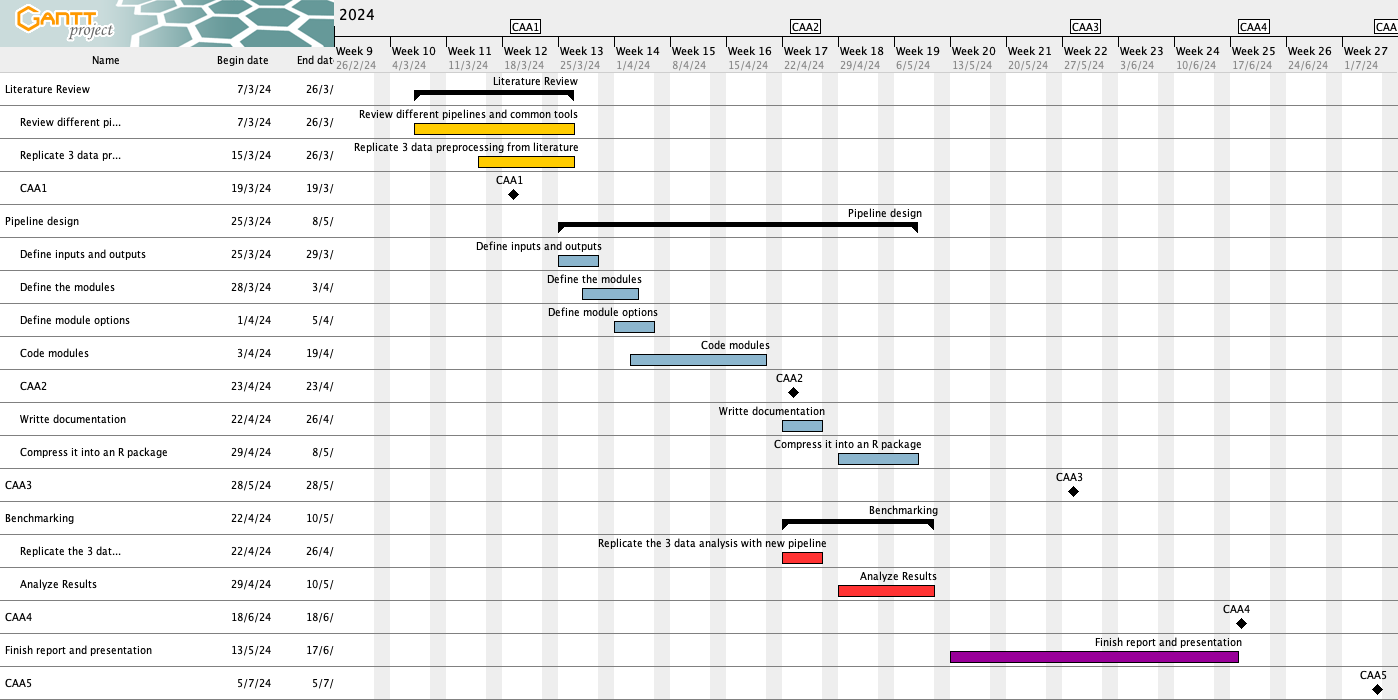
\includegraphics[width=\textwidth]{Images/gantt.png}
    \caption{Gantt chart showing the project timeline and milestones.}
    \label{fig:gantt}
\end{figure}

% \definecolor{gblue}{RGB}{66,133,244}
% \definecolor{gred}{RGB}{234,67,53}
% \definecolor{gyellow}{RGB}{251,188,4}
% \definecolor{ggreen}{RGB}{52,168,83}
% \definecolor{ggrey}{RGB}{154,160,166}
% \definecolor{gblack}{RGB}{32,33,36}
% \definecolor{gorange}{RGB}{227,116,0}

% \begin{landscape}
% \begin{ganttchart}[
%     % expand chart=\textwidth,
%     inline,
%     x unit = 10mm,
%     y unit title=0.5cm,
%     y unit chart=0.5cm,
%     time slot format=isodate-yearmonth,
%     time slot unit=day,
%     % calendar week text={W\currentweek},
%     title/.append style={shape=rectangle, fill=ggrey},
%     title height=1,
%     bar/.append style={fill=gyellow},
%     bar height=.6,
%     bar label font=\normalsize\color{gblack},
%     group top shift=.6,
%     group height=.3,
%     group peaks height=.2,
%     bar incomplete/.append style={fill=ggreen}
% ]{2024-03-05}{2024-07-15}
% \gantttitlecalendar{year, month, day} \\
% \ganttgroup{Literature Review}{2024-03-07}{2024-03-26} \\
%     \ganttbar{Review different pipelines and common tools}{2024-03-07}{2024-03-26}  \\
%     \ganttbar{Replicate 3 data preprocessing from literature}{2024-03-15}   {2024-03-26} \\
%     \ganttmilestone{CAA1}{2024-03-19}{2024-03-19} \\
% \ganttset{bar/.append style={fill=gblue}}
% \ganttgroup{Pipeline design}{2024-03-25}{2024-05-15} \\
%     \ganttbar{Define inputs and outputs}{2024-03-25}{2024-03-29} \\
%     \ganttbar{Define the modules}{2024-03-28}{2024-04-03} \\
%     \ganttbar{Define module options}{2024-04-01}{2024-04-05} \\
%     \ganttbar{Code modules}{2024-04-03}{2024-04-26} \\
%     \ganttbar{Code report}{2024-04-29}{2024-05-06} \\
%     \ganttmilestone{CAA2}{2024-04-23}{2024-04-23} \\
%     \ganttbar{Write documentation}{2024-05-06}{2024-05-15} \\
%     \ganttmilestone{CAA3}{2024-05-28}{2024-05-28} \\

% \ganttset{bar/.append style={fill=gred}}
% \ganttgroup{Benchmarking}{2024-05-13}{2024-05-20} \\
%     \ganttbar{Replicate the 3 data analysis with new pipeline}{2024-05-13}  {2024-05-14} \\
%     \ganttbar{Analyze Results}{2024-05-15}{2024-05-20} \\
%     \ganttmilestone{CAA4}{2024-06-18}{2024-06-18} \\
%     \ganttbar{Finish report and presentation}{2024-05-20}{2024-06-17} \\
%     \ganttmilestone{CAA5}{2024-07-05}{2024-07-05} \\
% \end{ganttchart}
% \end{landscape}
% \restoregeometry

\subsection{Tasks}
\subsubsection{Main Tasks and prioritization}
    \begin{enumerate}
        \item \textbf{Definition of the work plan:} Define the project's scope, objectives, methodology and expected outcomes. Create a project charter outlining the project's purpose and goals as well as a calendar with milestones and dates.
        \item \textbf{Literature review:} Review multiple publications and replicate the data processing from 3 of them. Review most used methods and tools for metabolomics data processing like normalization, scaling, filtering, transformation, batch effect
        \item \textbf{Pipeline design:} Propose and code in R a new pipeline to manage the processing of targeted metabolomics data.
        \item \textbf{Benchmarking:} Replicate again the data processing of the 3 publications using the new pipeline and compare the results.
    \end{enumerate}

    

\subsubsection{Extra tasks}
    \begin{enumerate}
        \item \textbf{Heavy-workload:} Optimize the pipeline to enable parallelization of the processing.
        \item \textbf{Documentation:} Write a documentation for the package so its accessibility.
        \item \textbf{R package implementation:} Pack the code for the pipeline in an R package to easy distribution.

    \end{enumerate}


\section{Risk analysis}

\begin{table}[!h]
    \centering
    \begin{tabular}{|c|c|c|p{6cm}|}
    \hline
    \rowcolor[HTML]{999999} 
    {\color[HTML]{FFFFFF} \textbf{Risk}} &
      {\color[HTML]{FFFFFF} \textbf{Severity}} &
      {\color[HTML]{FFFFFF} \textbf{Likelihood}} &
      \multicolumn{1}{c|}{\cellcolor[HTML]{999999}{\color[HTML]{FFFFFF} \textbf{Mitigation}}} \\ \hline
    \textbf{Resource constraints} &
      \cellcolor[HTML]{FFE599}Moderate &
      \cellcolor[HTML]{FFE599}Moderate &
      Develop a clear project timeline, incorporating milestones and allocating adequate time for each phase. Ensure contingency measures are in place to address unforeseen challenges or changes. \\ \hline
    \textbf{Technical challenges} &
      \cellcolor[HTML]{FFE599}Moderate &
      \cellcolor[HTML]{EA9999}High &
      Perform proper exploration of packages and software and seek guidance and mentorship from professors or experts in relevant fields. \\ \hline
    \textbf{User adoption and awareness} &
      \cellcolor[HTML]{EA9999}High &
      \cellcolor[HTML]{FFE599}Moderate &
      Be sure to incorporate appropriate cautions regarding the correct application of the chosen modules and data. \\ \hline
    \textbf{Pipeline branching} &
      \cellcolor[HTML]{B6D7A8}Low &
      \cellcolor[HTML]{FFE599}Moderate &
      Adopt new methods to interactively select the branching \\ \hline
    \end{tabular}
    \caption{Risk analysis. This table presents various risks associated with the project, along with
    their severity, likelihood, and potential mitigation measures.}
    \label{tab:risk-analysis}
\end{table}



\section{Final products}
\begin{itemize}
    \item A \textbf{pipeline} for targeted metabolomic data preprocessing designed to streamline data pretreatment tasks, optimize workflows, and ensure reproducibility in metabolomic research endeavors.
    \item A \textbf{R package} crafted to facilitate the seamless integration and modular implementation of the pipeline within the R environment, empowering researchers with flexible and efficient tools for metabolomic data analysis.
    \item A detailed \textbf{documentation} accompanying the pipeline and R package.
    \item A user-friendly \textbf{Shiny app} that enables researchers with varying levels of computational expertise to effortlessly pretreat targeted metabolomic data.
    % \item A public \textbf{repository} with the projects deliverables, source code of the package and the documentation. Thus encouraging transparency, collaboration, and community-driven enhancements to advance the state-of-the-art in metabolomic data preprocessing.
    \item A \textbf{PDF report} detailing the project's processes, including investigation, development, results, conclusions, and discussions.
    \item A \textbf{virtual presentation} providing a comprehensive overview of the project. This includes a video recording with explanatory narration to further enhance understanding.
\end{itemize}


\chapter{Materials and methods} \todo{Metodes: Com Desenvolupo // Materials: Amb que ho fas}

\section{Literature review}
The literature selected for the review was obtained from multiple journals. The search was conducted using the following keywords: "metabolomics", "data preprocessing", "data pretreatment", "metabolomics pipeline", "metabolomics tools", "metabolomics R packages", "targeted metabolomics", "nutrimetabolomics", "metabolomics proce". The search was limited to articles published in the last 20 years, with a focus on metabolomics data preprocessing and pretreatment methodologies. The review aimed to identify the most commonly used methods and tools for metabolomic data preprocessing and pretreatment, as well as to explore recent advancements in the field. The review also sought to identify gaps in the existing literature and to inform the development of the new pipeline.
\todo{Incloure taula amb els articles revisats?}

\section{Pipeline design}
The methods selected to be included in the pipeline were based on the results of the literature review. The pipeline was designed to be as modular as possible so a variety of methods are included to perform the same step, allowing users to select and apply specific pretreatment steps according to the data caracteristics and user needs and preferences.

\section{Datasets}
The datasets employed for the purpose of this study were obtained from public repositories. The datasets were selected based on the following criteria:
\begin{itemize}
    \item Aim of the dataset
    \item Availability of raw data
    \item Targeted metabolomics data
    \item Diverse biological samples
\end{itemize}

The datasets selected were 2:
\begin{itemize}
    \item \textbf{MTBLS79:} \cite{kirwanDirectInfusionMass2014} This dataset represents a systematic evaluation of the reproducibility of a multi-batch direct-infusion mass spectrometry (DIMS)-based metabolomics study of cardiac tissue extracts. It comprises twenty biological samples (cow vs. sheep) that were analysed repeatedly, in 8 batches across 7 days, together with a concurrent set of quality control (QC) samples. Data are presented from each step of the data processing workflow and are available through MetaboLights. This dataset was selected due to its importance in the field of metabolomics and its data aviability.
    \item \textbf{ST000284:} \cite{zhuColorectalCancerDetection2014} This dataset from MetaboWorkbench includes a study on colorectal cancer (CRC) using targeted liquid chromatography-tandem mass spectrometry. It examines 158 metabolites across 25 pathways in 234 serum samples (66 CRC patients, 76 polyp patients, 92 healthy controls). Blood samples were collected after fasting and bowel preparation. This dataset was selected due to its data aviability, its diversity (3 groups) and amount of samples.
    
\end{itemize}


\section{Packages}
The pipeline was developed using the R programming language \cite{R} and the packages described in \ref{tab:packages}.

\begin{table}[!h]
    \centering
    \begin{tabular}{@{}
    >{\columncolor[HTML]{FFFFFF}}l 
    >{\columncolor[HTML]{FFFFFF}}l 
    >{\columncolor[HTML]{FFFFFF}}c @{}}
    \toprule
    \multicolumn{1}{c}{\cellcolor[HTML]{FFFFFF}\textbf{Package}} & \multicolumn{1}{c}{\cellcolor[HTML]{FFFFFF}\textbf{Version}} & \textbf{Ref}                   \\ \midrule
    {\color[HTML]{000000} arrow}          & {\color[HTML]{000000} \textit{15.0.1}}  & \cite{R-arrow} \\
    {\color[HTML]{000000} base}           & {\color[HTML]{000000} \textit{4.3.3}}   & \cite{R}  \\
    {\color[HTML]{000000} BiocStyle}      & {\color[HTML]{000000} \textit{2.30.0}}  & \cite{R-BiocStyle}  \\
    {\color[HTML]{000000} caret}          & {\color[HTML]{000000} \textit{6.0.94}}  & \cite{R-caret}  \\
    {\color[HTML]{000000} cowplot}        & {\color[HTML]{000000} \textit{1.1.3}}   & \cite{R-cowplot}  \\
    {\color[HTML]{000000} crew}           & {\color[HTML]{000000} \textit{0.9.2}}   & \cite{R-crew}  \\
    {\color[HTML]{000000} datasets}       & {\color[HTML]{000000} \textit{4.3.3}}   & \cite{R}  \\
    {\color[HTML]{000000} dplyr}          & {\color[HTML]{000000} \textit{1.1.4}}   & \cite{R-dplyr}  \\
    {\color[HTML]{000000} DT}             & {\color[HTML]{000000} \textit{0.33}}    & \cite{R-DT}  \\
    {\color[HTML]{000000} fst}            & {\color[HTML]{000000} \textit{0.9.8}}   & \cite{R-fst}  \\
    {\color[HTML]{000000} ggforce}        & {\color[HTML]{000000} \textit{0.4.2}}   & \cite{R-ggforce}  \\
    {\color[HTML]{000000} graphics}       & {\color[HTML]{000000} \textit{4.3.3}}   & \cite{R-graph}  \\
    {\color[HTML]{000000} grDevices}      & {\color[HTML]{000000} \textit{4.3.3}}   & \cite{R}  \\
    {\color[HTML]{000000} HotellingEllipse}                      & {\color[HTML]{000000} \textit{1.1.0}}                        & \cite{R-HotellingEllipse} \\
    {\color[HTML]{000000} impute}         & {\color[HTML]{000000} \textit{1.76.0}}  & \cite{R-impute}  \\
    {\color[HTML]{000000} imputeLCMD}     & {\color[HTML]{000000} \textit{2.1}}     & \cite{R-imputeLCMD}  \\
    {\color[HTML]{000000} knitr}          & {\color[HTML]{000000} \textit{1.46}}    & \cite{R-knitr}  \\
    {\color[HTML]{000000} MetaboAnalystR} & {\color[HTML]{000000} \textit{4.0.0}}   & \cite{R-MetaboAnalystR}  \\
    {\color[HTML]{000000} methods}        & {\color[HTML]{000000} \textit{4.3.3}}   & \cite{R}  \\
    {\color[HTML]{000000} missForest}     & {\color[HTML]{000000} \textit{1.5}}     & \cite{R-missForest}  \\
    {\color[HTML]{000000} pcaMethods}     & {\color[HTML]{000000} \textit{1.94.0}}  & \cite{R-pcaMethods}  \\
    {\color[HTML]{000000} pmp}            & {\color[HTML]{000000} \textit{1.14.1}}  & \cite{R-pmp}  \\
    {\color[HTML]{000000} purrr}          & {\color[HTML]{000000} \textit{1.0.2}}   & \cite{R-purrr}  \\
    {\color[HTML]{000000} renv}           & {\color[HTML]{000000} \textit{1.0.7}}   & \cite{R-renv}  \\
    {\color[HTML]{000000} reshape2}       & {\color[HTML]{000000} \textit{1.4.4}}   & \cite{R-reshape2}  \\
    {\color[HTML]{000000} rmarkdown}      & {\color[HTML]{000000} \textit{2.27}}    & \cite{R-rmarkdown}  \\
    {\color[HTML]{000000} shiny}          & {\color[HTML]{000000} \textit{1.8.1.1}} & \cite{R-shiny}  \\
    {\color[HTML]{000000} shinyFiles}     & {\color[HTML]{000000} \textit{0.9.3}}   & \cite{R-shinyFiles}  \\
    {\color[HTML]{000000} stats}          & {\color[HTML]{000000} \textit{4.3.3}}   & \cite{R}  \\
    {\color[HTML]{000000} structToolbox}  & {\color[HTML]{000000} \textit{1.14.0}}  & \cite{R-structToolbox}  \\
    {\color[HTML]{000000} SummarizedExperiment}                  & {\color[HTML]{000000} \textit{1.32.0}}                       & \cite{R-SummarizedExperiment} \\
    {\color[HTML]{000000} tarchetypes}    & {\color[HTML]{000000} \textit{0.9.0}}   & \cite{R-tarchetypes}  \\
    {\color[HTML]{000000} targets}        & {\color[HTML]{000000} \textit{1.7.0}}   & \cite{R-targets}  \\
    {\color[HTML]{000000} tidyverse}      & {\color[HTML]{000000} \textit{2.0.0}}   & \cite{R-tidyverse}  \\
    {\color[HTML]{000000} tinytex}        & {\color[HTML]{000000} \textit{0.51}}    & \cite{R-tinytex}  \\
    {\color[HTML]{000000} tools}          & {\color[HTML]{000000} \textit{4.3.3}}   & \cite{R}  \\
    {\color[HTML]{000000} usethis}        & {\color[HTML]{000000} \textit{2.2.3}}   & \cite{R-usethis}  \\
    {\color[HTML]{000000} utils}          & {\color[HTML]{000000} \textit{4.3.3}}   & \cite{R}  \\
    {\color[HTML]{000000} VIM}            & {\color[HTML]{000000} \textit{6.2.2}}   & \cite{R-VIM}  \\
    {\color[HTML]{000000} withr}          & {\color[HTML]{000000} \textit{3.0.0}}   & \cite{R-withr}  \\ \bottomrule
    \end{tabular}
    \caption{List of R packages with their versions used to develop \texttt{metaboPipe}}
    \label{tab:packages}
    \end{table}


    
    
    
    
    
\chapter{Results} \todo{add a summary of 1: Number of functions and 2: Number of lines of code}

\section{Pipeline}
The literature review provided valuable insights into the most commonly used methods and tools for metabolomic data preprocessing. Based on this information, the proposed pipeline is designed to include the following steps:
\begin{figure}[ht]
    \centering
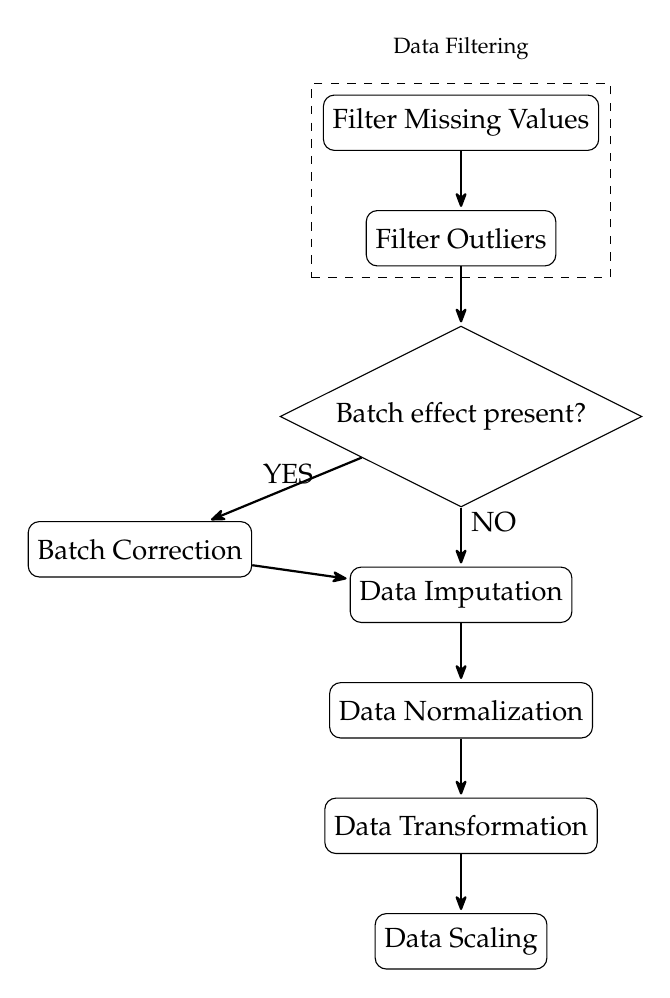
\begin{tikzpicture}[node distance=.75cm and .5cm]

    % Subgraph: Data Filtering
    \node[block] (A) {Filter Missing Values};
    \node[block, below=of A] (B) {Filter Outliers};
    
    \node[decision, below=of B] (C) {Batch effect present?};
    \node[block, below left=of C, xshift=-1cm] (D) {Batch Correction};
    \node[block, below=of C] (H) {Data Imputation};
    \node[block, below=of H] (E) {Data Normalization};
    \node[block, below=of E] (F) {Data Transformation};
    \node[block, below=of F] (G) {Data Scaling};
  
    % Arrows
    \path [line] (A) -- (B);
    \path [line] (B) -- (C);
    \path [line] (C) -- node[near start, left] {YES} (D);
    \path [line] (C) -- node[near start, right] {NO} (H);
    \path [line] (D) -- (H);
    \path [line] (H) -- (E);
    \path [line] (E) -- (F);
    \path [line] (F) -- (G);
  
    % Subgraph label
    \node[draw=black, dashed, fit=(A)(B), inner sep=4pt, label={[label distance=0.5em]north:Data Filtering}] {};
  
  \end{tikzpicture}
  \caption{Flow diagram showing the steps of the metabolomic data preprocessing pipeline proposed.}
  \label{fig:pipeline}
\end{figure}
  
In this project, an R package named \texttt{metaboPipe} was developed to preprocess metabolomic data efficiently and accessibly. Metabolomic data preprocessing is a crucial step in ensuring the quality and reliability of downstream analyses. The transformations applied during preprocessing are primarily intended to remove unwanted effects unrelated to the study, but these tools can inadvertently delete meaningful biological data if used without caution. The \texttt{metaboPipe} package leverages the \texttt{targets} and \texttt{structToolbox} packages to create a modular and reproducible pipeline for preprocessing. This section details the components and functionality of \texttt{metaboPipe}.

\section{Package Overview}
The \texttt{metaboPipe} package is designed to streamline the preprocessing of metabolomic data by creating a series of user-accessible modules that translate into interconnected steps. These steps can be easily added, modified, and rearranged. The package utilizes the \texttt{targets} package to orchestrate task deployment and dependencies, ensuring that each step is executed in the correct order. The \texttt{structToolbox} package provides the \texttt{DatasetExperiment} object, which serves as the primary data structure throughout the pipeline, along with multiple functions for data transformation.

The package can be divided into three main categories:
\begin{itemize}
    \item \textbf{Data manipulation:} These functions are the core of the package, as they transform the data into the desired formats and apply the diversity of methods to perform the preprocessing steps including the visualization.
    \item \textbf{Target factories:} They are the pipeline contruction functions for the users to interact with, as they use the targets package to create pipeline nodes that use the data manipulation functions. Each factory is intended to represent a specific pretreatement step.
    \item \textbf{Shiny app:} This is a user-friendly interface that allows users to create and run the pipeline without the need for R programming knowledge.
\end{itemize}

\section{Data manipulation}
For the pretreatement of the data, the package includes the following functions:

\begin{itemize}    
    \item A function to create a \texttt{DatasetExperiment} object from a list of dataframes.
    \item A function to filter the data based on the percentage of missing values both in the features and the samples.  
    \item A function to filter the outliers based on a Hotelling's T2 distribution ellipse.
    \item 8 functions to impute the missing values based on the following methods: \textit{Mean, Median, Random Forest (RF), Quantile Regression Imputation of Left-Censored data (QRILC), k-Nearest Neighbors (kNN), Singular Value Decomposition (SVD), Bayesian Principal Component Analysis (BPCA) and Probabilistic Principal Component Analysis (PPCA)}.
    \item 2 functions to remove the batch effect using either the \textit{Quality Control-Robust Spline Correction (QC-RSC)} method or the \texttt{ComBat} method. \todo{add references to the methods}
    \item A function to normalize, scale and transform the data based on the methods provided by the \texttt{metaboAnalystR} package.
    \item 12 data visualization functions to create plots. 
    \item 17 utility functions to perform different tasks. 
\end{itemize}
    

\section{Target factories}
For the pipeline construction, the package includes the following 9 functions:
\begin{itemize}
    \item The \texttt{load\_data} function is implemented to efficiently load and read data from specified files into data frames. It dynamically creates six different nodes based on the presence of the \texttt{variableMetadata} parameter.
    \item The \texttt{create\_experiment} function is the pivotal component in the data processing pipeline, enabling the creation of a \texttt{DatasetExperiment} S4 object that will be used in almost all of the pipeline. This facilitates efficient modularity.
    \item The \texttt{factorize\_cols} function that makes the specified columns of the \texttt{sampleMetadata} as factors.
    \item The \texttt{filter\_step} function that creates up to 5 nodes depending on the parameters provided. These nodes filter the data based on the percentage of missing values in the features and samples, filter outliers using a Hotelling's T2 distribution ellipse and creates a plot for visualizing the data missing values before and after the filtering is done.
    \item The \texttt{batch\_correct} function that creates a node to remove the batch effect using the \texttt{QC-RSC} method.
    \item The \texttt{impute} function that creates a node to impute the missing values using the method provided.
    \item The \texttt{normalize} function that creates a node to normalize, scale and/or transform the data using the methods provided.
    \item The \texttt{export\_data} function that creates a node to export the data to a specified directory.
\end{itemize}

\section{Documentation}
The package is distributed with documentation that consists of three parts:
\begin{itemize}
    \item The help documentation for the methods and functions of the package.
    \item A PDF manual that includes all the aforementioned methods and functions of the package.
    \item A tutorial vignette that details the processing of the ST000284 dataset using the package to create and execute a pipeline.
\end{itemize}

\section{Shiny app}
% https://i.imgur.com/LQB1z2B.png
% https://i.imgur.com/1ZeEmNK.png
% https://i.imgur.com/gGDcwui.png

A shiny app was developed to allow users to interact with the pipeline without the need for R programming knowledge. The app provides 3 main tabs:
\begin{itemize}
    \item The \texttt{Data upload} tab allows users to either upload their data or use one of the example data provided.
    \item The \texttt{Data Config} tab allows users to set the global parameters for the data, like the sample\_ID column, the column to be used as QC or Sample identifier, and the main study factor. It also allows users to visualize the data tables they are working with to ensure the data is correctly loaded.
    \item The \texttt{Process Selector} tab allows users to select and configure the different steps of the pipeline. Each step is represented by a card that can be expanded to show the parameters of the step. The user can select the steps they want to include in the pipeline and configure them according to their needs. The app will then generate the \texttt{\_targets.R} file and execute the pipeline from the app.
\end{itemize}

\chapter{Discussion}
Different methods for preprocessing metabolomic data are essential to accommodate the diverse types of data encountered in this field. This variety arises due to the numerous factors influencing metabolomic data, which can be biological, technical, or experimental. Each preprocessing method offers unique advantages and disadvantages. Therefore, choosing the appropriate method can be challenging and is guided by the specific biological question, the nature of the data, and the desired analytical outcomes.

In this work, a general workflow for targeted metabolomics data preprocessing has been proposed. This workflow is not specific as the selection of preprocessing methods affects their order. For example, when using singular value decomposition (SVD) as an imputation method, it is recommended to scale and center the data beforehand, but if we impute the data using quantile regression imputation of left-censored data (QRILC), log-transforming the data beforehand is recommended for better accuracy \todo{38}. When normalizing Quantile normalization (QN) is not recomended for datasets with $n < 50$ samples \todo{67} and Probabilistic Quotient Normalization (PQN) is not adequate to use when the number of metabolites is $>$ than the number of samples \todo{59}.
These considerations must be factored in when selecting preprocessing methods, making it impractical to establish a one-size-fits-all pipeline

Due to the diversity of methods and their interactions, this work focuses on developing a tool that facilitates the easy and interactive creation of customized data preprocessing sequences. This tool, the \texttt{metaboPipe} package, offers functions to perform common preprocessing steps and enables the creation of tailored pipelines using these steps. Additionally, the package includes a shiny app that allows users to interact with the pipeline without requiring R programming skills.

To load the data, users need to import two tables in \texttt{.csv} format: \texttt{dataMatrix} and \texttt{sampleMetadata}. The \texttt{dataMatrix} table contains the relative abundance or concentration data (\Cref{tab
}), while the \texttt{sampleMetadata} table holds the sample-related data (\Cref{tab
}).


% DataMatrix table
\begin{table}[htbp]
    \centering
    \caption{A data matrix generated by a metabolomics platform}
    \label{tab:dataMatrix-example}
    \begin{tabular}{@{}lllll@{}}
      \toprule
      \multicolumn{1}{c}{$n \times m$} & \multicolumn{1}{c}{$Metabolite_1$} & \multicolumn{1}{c}{$Metabolite_2$} & \multicolumn{1}{c}{$\dots$} & \multicolumn{1}{c}{$Metabolite_m$} \\ \midrule
      $Sample_1$ &  &  &  &  \\
      $Sample_2$ &  &  &  &  \\
      \multicolumn{1}{c}{$\dots$} & \multicolumn{1}{c}{$\dots$} & \multicolumn{1}{c}{$\dots$} & \multicolumn{1}{c}{$\dots$} & \multicolumn{1}{c}{$\dots$} \\ 
      $Sample_n$ &  &  &  &  \\ \bottomrule
    \end{tabular}
  \end{table}
% sampleMetadata table
  \begin{table}[htbp]
    \centering
    \caption{The sampleMetadata matrix generated by a metabolomics platform}
    \label{tab:sampleMetadata-example}
    \begin{tabular}{@{}lllll@{}}
      \toprule
      \multicolumn{1}{c}{$n \times m$} & \multicolumn{1}{c}{$Factor_1$} & \multicolumn{1}{c}{$Factor_2$} & \multicolumn{1}{c}{$\dots$} & \multicolumn{1}{c}{$Factor_m$} \\ \midrule
      $Sample_1$ &  &  &  &  \\
      $Sample_2$ &  &  &  &  \\
      \multicolumn{1}{c}{$\dots$} & \multicolumn{1}{c}{$\dots$} & \multicolumn{1}{c}{$\dots$} & \multicolumn{1}{c}{$\dots$} & \multicolumn{1}{c}{$\dots$} \\ 
      $Sample_n$ &  &  &  &  \\ \bottomrule
    \end{tabular}
  \end{table}
    
  

  For filtering missing values, the modified 80\% rule is adopted by default: if a column or row has more than 20\% missing values, that column or row is removed. Users can manually adjust the threshold for missing values.

  To identify and filter outliers, a Hotelling's T2 distribution ellipse is used with a default significance level of 95\%, adjustable to 99\% if desired. This method is chosen for its robustness and flexibility in detecting outliers in multivariate data, considering the covariance between variables \cite{wuUsingNontargetedLCMS2021, viallonNewPipelineNormalization2021}.
  
  Batch effects are a common issue in metabolomics studies, introducing unwanted variability into the data. To correct this effect, two methods have been implemented: the \texttt{QC-RSC} method and the \texttt{ComBat} method, which are widely used \todo{add citations}.
  
  
  
  For normalization, scaling, and transformation of the data, it has been decided to use the methods provided by the \texttt{metaboAnalystR} package as it offers a wide variety of methods, some of which are difficult to implement manually, such as normalization to an internal standard or a physiological constant. However, several functions are implemented to normalize the data using other methods not present in \texttt{metaboAnalystR} such as Probabilistic Quotient Normalization (PQN) or Vector Length Normalization (VLN). These methods, although implemented in \texttt{metaboPipe}, are not incorporated into the shiny application interface nor the \texttt{normalize()} function.
  
  The implementation of the PC-PR2 method described by \citeauthor{viallonNewPipelineNormalization2021} is also considered. This method first identifies sources of variation using PCA combined with multiple linear regression and then corrects unwanted variations using a random effects model for each metabolite. However, due to the complexity of robustly integrating this method into the package within the available time, it is deferred to future revisions. Nevertheless, the \texttt{pcpr2()} function can be used to visualize the data and identify sources of variation, although correction is not yet possible.
  



\chapter{Conclusion and future vision}
The second one is that it enables the pipeline to be used as a pretreatement method comparable tool. As the easy of use and order can be easily changed, the user can test different pretreatement methods and orders to compare the changes in the data.

%\section{Conclusiones}
Este capítulo tiene que incluir:
\begin{itemize}
\item Una descripción de las conclusiones del trabajo:
\begin{itemize}
    \item Una vez se han obtenido los resultados, ¿qué conclusiones se extraen?
    \item ¿Estos resultados son los esperados? ¿O han sido sorprendentes? ¿Por qué? 
\end{itemize}
\item Una reflexión crítica sobre el logro de los objetivos planteados inicialmente:
\begin{itemize}
    \item ¿Hemos logrado todos los objetivos? Si la respuesta es negativa, ¿por qué motivo?
\end{itemize}
\item Un análisis crítico del seguimiento de la planificación y metodología a lo largo del producto:
\begin{itemize}
    \item ¿Se ha seguido la planificación?
    \item ¿La metodología prevista ha sido suficientemente adecuada?
    \item ¿Ha habido que introducir cambios para garantizar el éxito del trabajo? ¿Por qué? 
\end{itemize}
\item De los impactos previstos en \ref{s:etic}, ético-sociales, de sostenibilidad y de diversidad, evaluar/mencionar si se han mitigado (si eran negativos) o si se han conseguido (si eran positivos). 
\item Si han aparecido impactos no previstos a \ref{s:etic}, evaluar/mencionar cómo se han mitigado (si eran negativos) o que han aportado (si eran positivos).
\item Las líneas de trabajo futuro que no se han podido explorar en este trabajo y han quedado pendientes.
\item Glossary test:  \gls{latex}


%\item Una descripción de las conclusiones del trabajo: Qué lecciones se han aprendido del trabajo?
%\item Una reflexión crítica sobre el logro de los objetivos planteados inicialmente: Hemos conseguido todos los objetivos? Si la respuesta es negativa, por qué motivo?
%\item De los impactos previstos a la sección \ref{s:etic}, una evaluación, o al menos, mención, sobre si se han mitigado (si eran negativos) o si se han conseguido (si eran positivos). 
\end{itemize}

%\section{Líneas de futuro}
%Las líneas de trabajo futuro que no se han podido explorar en este trabajo y han quedado pendientes.

%\section{Seguimiento de la planificación}
%Un análisis crítico del seguimiento de la planificación y metodología a lo largo del trabajo: 
%\begin{itemize}
%    \item  Se ha seguido la planificación? 
%    \item La metodología prevista ha sido la adecuada? 
%    \item Ha habido que introducir cambios para garantizar el éxito del trabajo? ¿Por qué? 
%\end{itemize}

\setglossarystyle{list}
\printglossary[title=Glossary, toctitle=Glossary]
\printglossary[type=\acronymtype, title=Acronyms, toctitle=Acronyms]



\printbibliography[heading=bibintoc]


\newpage
\appendix
Listado de apartados que son demasiado extensos para incluir dentro de la memoria y tienen un carácter autocontenido (por ejemplo, manuales de usuario, manuales de instalación, etc.)
 
Dependiendo del tipo de trabajo, es posible que no haya que añadir algún anexo.

\end{document}
